\documentclass[hyperref={pdfpagelabels=true}]{beamer}

\usepackage{lmodern}

\title{Bases de Dados Espaciais}   
\author{Joana Sim\~{o}es} 
\date{\today} 
 
\usepackage{beamerthemeshadow}
%\usepackage{beamerthemesplit}
\usepackage{listings}

\newcommand{\soooo}{H$_2$SO$_4$}

\begin{document}
\setbeamertemplate{footline}[page number]
\setbeamertemplate{navigation symbols}{}
\begin{frame}
\titlepage
\end{frame} 

\begin{frame}
\frametitle{Table of contents}
\tableofcontents
\end{frame}
 

\section{Introducao} 
\begin{frame}
\frametitle{Apresentacao}
\begin{columns}
  \begin{column}{7cm}
    \begin{itemize}
      \item<1-> PhD CASA, UCL: "An Agent-based Approach to Epidemics through GIS"
      \item<2-> membro do grupo de ``Modelacao Geografica, Cidades e Ordenamento Do Territorio'', e-GEO
      \item<3-> + 2 anos na FAO-UN, como consultora de diversos aspectos relacionados com Software (programacao, Bases de Dados e SIG)
      \end{itemize}
  \end{column}
  \begin{column}{10cm}
    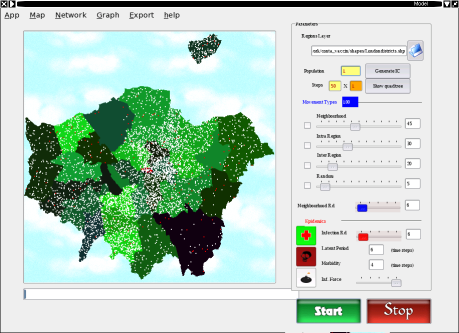
\includegraphics[scale=0.4]{input1.png}
  \end{column}  
\end{columns}
\end{frame}


\begin{frame}
\frametitle{Motivacao para Este Talk/Workshop}
\end{frame}

\begin{frame}
\frametitle{O que este Talk nao e...}
\end{frame}

\section{Conceitos Gerais de Base de Dados}
\subsection{BD como Modelos de Realidade}
\begin{frame}
\frametitle{O que sao Bases de Dados...?}
\begin{overprint}
\begin{figure}
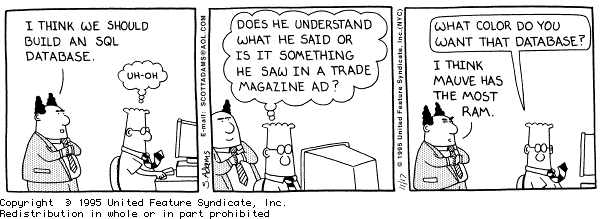
\includegraphics[scale=0.4]{dilbert_db.png}
\end{figure}
\end{overprint}
\end{frame}

\begin{frame}
\frametitle{O que sao Bases de Dados...? (+)}
\begin{columns}
  \begin{column}{7cm}
    \begin{itemize}
      \item<2-> As BD tratam de organizar a informacao;
      \item<3-> Exemplos de BD: arquivo de uma biblioteca, folha de calculo ou ficheiro de texto;
    \end{itemize}
  \end{column}
  \begin{column}{10cm}
    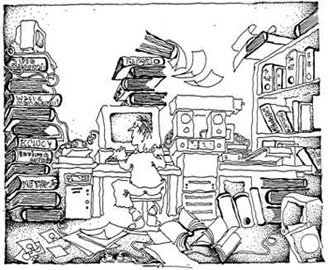
\includegraphics[scale=0.4]{informationoverloadcartoon.jpg}
  \end{column}  
\end{columns}
\end{frame}

\begin{frame}
\frametitle{O que sao Bases de Dados...? (+)}
\begin{overprint}
\begin{figure}
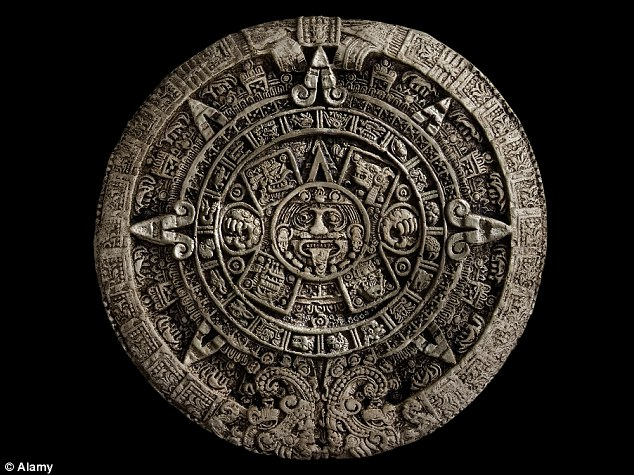
\includegraphics[scale=0.4]{mayas.jpg}
\end{figure}
Calendario Maya.\\
\end{overprint}
\end{frame}

\begin{frame}
\frametitle{O que sao Bases de Dados...? (+)}
\begin{overprint}
Os computadores/Internet geram um volume de dados muito grande e necessitamos de ferramentas adequadas para tirar partido deles.\\
\begin{figure}
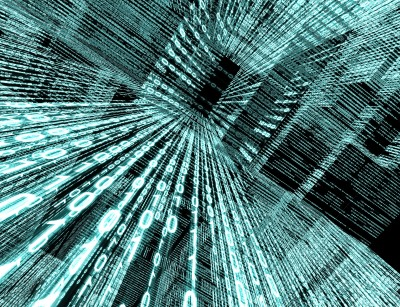
\includegraphics[scale=0.4]{Big-Data-on-cloud.jpg}
\end{figure}
\end{overprint}
\textit{Cloud Computing; Data Mining; Grid Computing; Data Warehouses; Big Data;}
\end{frame}

\subsection{BD Relacionais}
\begin{frame}
\frametitle{BD Relacionais}
O modelo relacional foi formulado por Edgar F. Codd (1969/1970?).\\
Este modelo representa a realidade atraves de: \textbf{tabelas}, \textbf{colunas} e \textbf{linhas}.
%\begin{columns}
  %\begin{column}{5cm}
  \begin{itemize}
  \item<2-> Os dados sao armazenados em \textbf{tabelas}.
  \item<3-> As tabelas sao organizadas por \textbf{colunas}; cada coluna guarda um \emph{tipo} de dados (inteiro, real, caracter, BLOB,...).  
  \item<4-> Os dados correspondentes a uma \textit{instancia} unica da tabela sao armazenados numa \textbf{linha}.
  \item<5-> As tabelas tipicamente apresentam \textbf{chaves} - uma ou mais colunas que identificam unicamente essa linha dentro da tabela.
  \item<6-> Para tornar o acesso a tabela mais rapido, e definido um \textbf{indice}. Um indice possibilita buscas rapidas na tabela, baseadas numa ou mais colunas (chave).
  \end{itemize}
  %\end{column}
%\end{columns}
\end{frame}

\begin{frame}
\frametitle{BD Relacionais (+)}
  \begin{figure}
  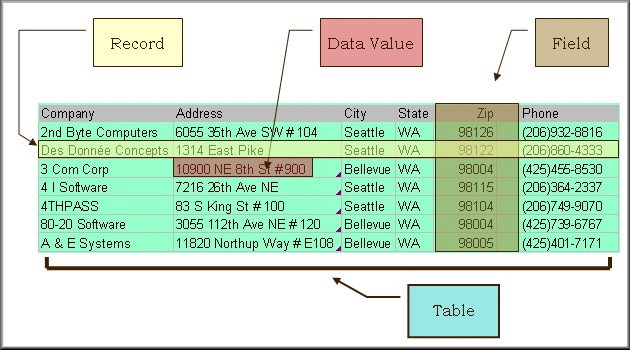
\includegraphics[scale=0.3]{table.png}
  \end{figure}
Relacao: conjunto de registos com os mesmos atributos (i.e.: mesmo dominio).\\
%Relacoes base e relacoes derivadas    
  \begin{figure}
  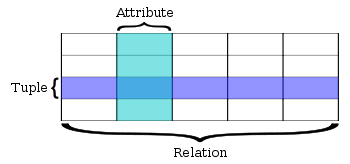
\includegraphics[scale=0.4]{350px-Relational_database_terms.png}
  \end{figure}
\end{frame}

\begin{frame}
\frametitle{BD Relacionais (+)}
Relacoes entre tabelas:\\
\begin{figure}
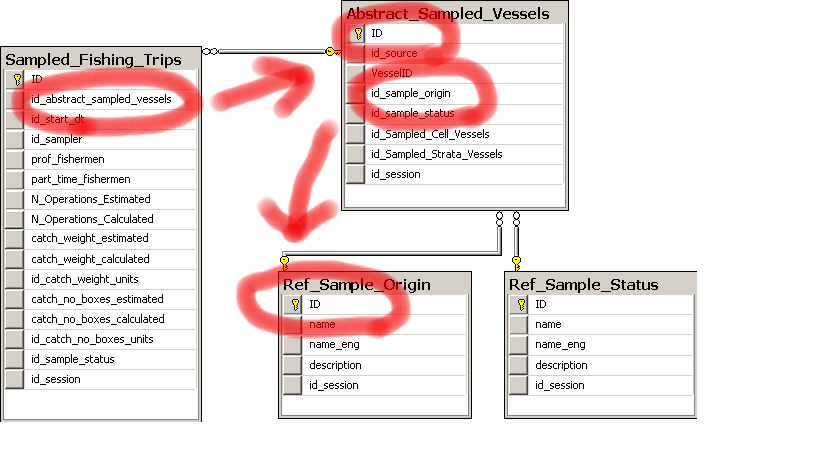
\includegraphics[scale=0.5]{sample_status_originb}
\end{figure}
\end{frame}

\begin{frame}
\frametitle{BD Relacionais (+)}
O objectivo do modelo relacional e possibilitar um metodo declarativo para especificar dados e \textit{queries}.
  \begin{enumerate}
  \item<2-> Os utilizadores declaram que informacao contem a BD e que informacao querem extrair dela.
  \item<3-> O software encarrega-se de descrever as estruturas de dados para armazenamento e os procedimentos de recuperacao dos dados para responder as \textit{queries}.
  \end{enumerate}
\end{frame}

\subsection{SQL}
\begin{frame}
\frametitle{SQL}
A maior parte das implementacoes do modelo relacional usam o \textbf{SQL} como linguagem de definicao de dados e de \textit{queries}.
  \begin{itemize}
  \item<2-> Linguagem estruturada de pesquisa (\textbf{S}tructured \textbf{Q}uery \textbf{L}anguage).
  \item<3-> Embora nao subscreva a 100\% o modelo proposto por Todd (1970) tornou-se a linguagem de BD mais utilizada.
  \item<4-> Originalmente baseada na algebra relacional, foi extendendo o seu ambito (e.g.: insercao de dados, pesquisa, actualizacao, remocao, etc)
  \end{itemize}
\end{frame}

\begin{frame}[fragile]
\frametitle{SQL (+)}
\lstset{language=SQL}
\begin{lstlisting}
SELECT * FROM STUDENTS WHERE YR 2012;
SELECT (1+1);
ALTER TABLE MyTable ADD myField4 NUMBER(3);
DROP DATABASE MYDB; 
\end{lstlisting}
\end{frame}

\begin{frame}[fragile]
\frametitle{SQL (+)}
\lstset{language=SQL}
\tiny{
\begin{lstlisting}
SELECT Ref_Vessels.Name	
FROM         dbo.FR_ALS2Vessel INNER JOIN
dbo.Ref_Vessels ON dbo.FR_ALS2Vessel.vesselID = dbo.Ref_Vessels.VesselID
WHERE     (dbo.FR_ALS2Vessel.id_sub_frame =
(SELECT     ID
FROM          dbo.FR_Sub_Frame
WHERE      (Type =
(SELECT     ID
FROM          dbo.Ref_Frame
WHERE      (Name = 'root'))) AND (id_frame = 8)))
AND (dbo.FR_ALS2Vessel.id_abstract_landingsite =
(SELECT     id_abstract_LandingSite
  FROM          dbo.Sampled_Cell
  WHERE      (ID = 53)))
AND (dbo.FR_ALS2Vessel.vesselID NOT IN
(SELECT     VesselID
FROM          dbo.Changes_Temp_Vessel
WHERE      (id_cell = 53) AND (To_LS =
(SELECT     ID
  FROM          dbo.Ref_Abstract_LandingSite
  WHERE      (Name = 'outside')))))
UNION
SELECT Ref_Vessels.Name	
FROM         dbo.FR_ALS2Vessel INNER JOIN
dbo.Ref_Vessels ON dbo.FR_ALS2Vessel.vesselID = dbo.Ref_Vessels.VesselID
WHERE     (dbo.Ref_Vessels.VesselID IN
(SELECT     VesselID
FROM          dbo.Changes_Temp_Vessel
WHERE      (id_cell = 53) AND (To_LS = 
(SELECT id_abstract_LandingSite FROM Sampled_Cell WHERE ID=53)							
)))
\end{lstlisting}
}
\end{frame}

\subsection{Sistemas de Gestao de Base de Dados}
\begin{frame}
\frametitle{SGBD}
Um \textbf{S}istema de \textbf{G}estao De \textbf{B}ase de \textbf{D}ados e o software que controla o armazenamento,
recuperacao, remocao, seguranca e integridade dos dados dentro da BD.\\
Algumas vantagens dos SGBDR:
\begin{itemize}
\item<2-> Reduzir a redundancia;%Bd centralizada; utilizacao de chaves estrangeiras
\item<3-> Independencia dos dados;%se a BD estiver separada da aplicacao, a aplicacao nao necessita de saber nada sobre o armazenamento interno, manipulacao dos dados
\item<4-> Assegurar a integridade dos dados;%ao activar certos mecanismos (por exemplo chaves primarias) a BD vai assegurar-se de que nao existem registos duplicados
\item<5-> Partilha de dados;%varias aplicacoes podem partilhar a mm BD
\item<7-> Recuperacao a partir de uma falha;%multiplos updates podem ser agrupados numa unica transaccao logica; o update fisico segue a compleicao da transaccao logica; desta forma, assegura-se que numa falha, a BD nao vai ficar num estado inconsistente
\item<8-> Seguranca e privacidade;%implementa sistema de utilizadores e roles, protegidos com passwords, permitindo varios niveis de acesso aos dados
\end{itemize}
\end{frame}

\section{Base de Dados Espaciais}

\subsection{O que sao as BD Espaciais} 
\begin{frame}
\frametitle{O que sao as BD Espaciais}
\end{frame}


\subsection{BD e SIG} 
\begin{frame}
\frametitle{BD e SIG}
\end{frame}


\subsection{Software Livre e de Codigo Aberto (FOSS)}
\begin{frame}
\frametitle{Software Livre e de Codigo Aberto (FOSS)}
\end{frame}

\subsection{Exemplos de SGBD com Extensoes Espaciais}
\begin{frame}
\frametitle{Exemplos de SGBD com Extensoes Espaciais}
\end{frame}

\end{document}
\begin{frame}
\frametitle{lists with single pause}
\begin{itemize}
\item keyword  \pause 
\item still another keyword
\end{itemize} 

\end{frame}

\begin{frame}
\frametitle{lists with pause}
\begin{itemize}[<+->]
\item keyword  
\item still another keyword
\item a third one 
\end{itemize} 
\end{frame}


\subsection{Lists II}
\begin{frame}
\frametitle{numbered lists}
\begin{enumerate}
\item keyword
\item still another keyword
\end{enumerate}
\end{frame}

\begin{frame}
\frametitle{numbered lists with single pause}
\begin{enumerate}
\item keyword  \pause 
\item still another keyword
\end{enumerate}
\end{frame}

\begin{frame}
\frametitle{numbered lists with pause}
\begin{itemize}[<+->]
\item keyword  
\item still another keyword
\item a third one 
\end{itemize} 
\end{frame}


\section{Section no.3} 
\subsection{Tables}
\begin{frame}
\frametitle{Tables}
\begin{tabular}{|l|c|r|p{1.5 cm }|}
\hline
left & centers & right & width \\
l & C & r & p \\
\hline
\end{tabular}
\end{frame}


\begin{frame}
\frametitle{Tables with pause}
\begin{tabular}{c c c}
A & B & C \\ 
\pause 
1 & 2 & 3 \\  
\pause 
A & B & C \\ 
\end{tabular} 
\end{frame}


\section{Section no. 4}
\subsection{blocs}
\begin{frame}
\frametitle{blocs}

\begin{block}{title of the bloc}
bloc text
\end{block}

\begin{exampleblock}{title of the bloc}
bloc text
\end{exampleblock}


\begin{alertblock}{title of the bloc}
bloc text
\end{alertblock}
\end{frame}


\section{Section no. 5}
\subsection{split screen}

\begin{frame}
\frametitle{splitting screen}
\begin{columns}
\begin{column}{5cm}
\begin{itemize}
\item Beamer 
\item Beamer Class 
\item Beamer Class Latex 
\end{itemize}
\end{column}
\begin{column}{5cm}
\begin{tabular}{|c|c|}
\hline
\textbf{Instructor} & \textbf{Title} \\
\hline
Sascha Frank &  \LaTeX \ Course 1 \\
\hline
Sascha Frank &  Course serial  \\
\hline
\end{tabular}
\end{column}
\end{columns}
\end{frame}

\subsection{Pictures} 
\begin{frame}
\frametitle{pictures in latex beamer class}
\begin{figure}
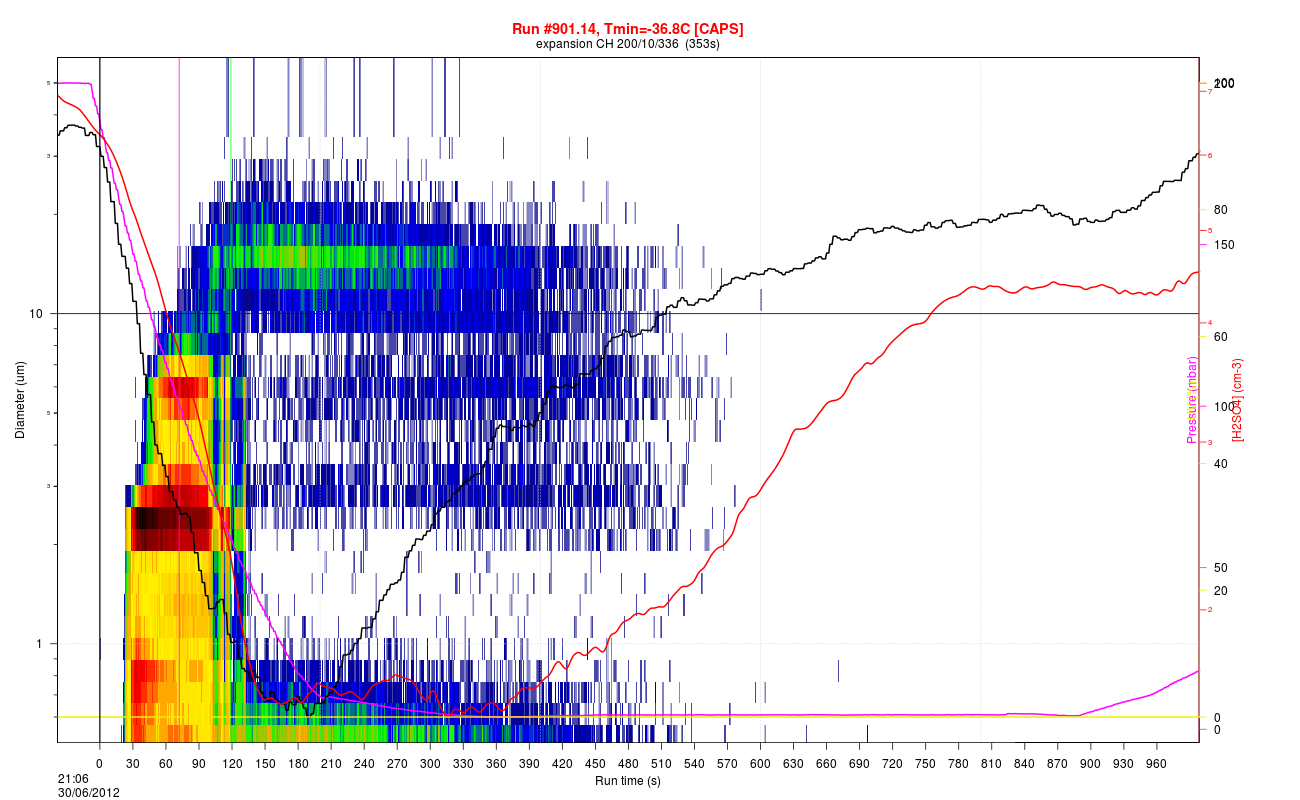
\includegraphics[scale=0.4]{runs_for_talk01.png} 
\caption{show an example picture}
\end{figure}
\end{frame}

\subsection{joining picture and lists} 

\begin{frame}
\frametitle{pictures and lists in beamer class}
\begin{columns}
\begin{column}{5cm}
\begin{itemize}
\item<1-> subject 1
\item<2-> subject 2
\item<3-> subject 3
\end{itemize}
\vspace{3cm} 
\end{column}
\begin{column}{5cm}
\begin{overprint}
\includegraphics<1>[scale=0.1]{runs_for_talk01.png}
\includegraphics<2>[scale=0.1]{runs_for_talk02.png}
\includegraphics<3>[scale=0.1]{runs_for_talk03.png}
\end{overprint}
\end{column}
\end{columns}
\end{frame}

\subsection{pictures which need more space} 
\begin{frame}[plain]
\frametitle{plain, or a way to get more space}
\begin{figure}
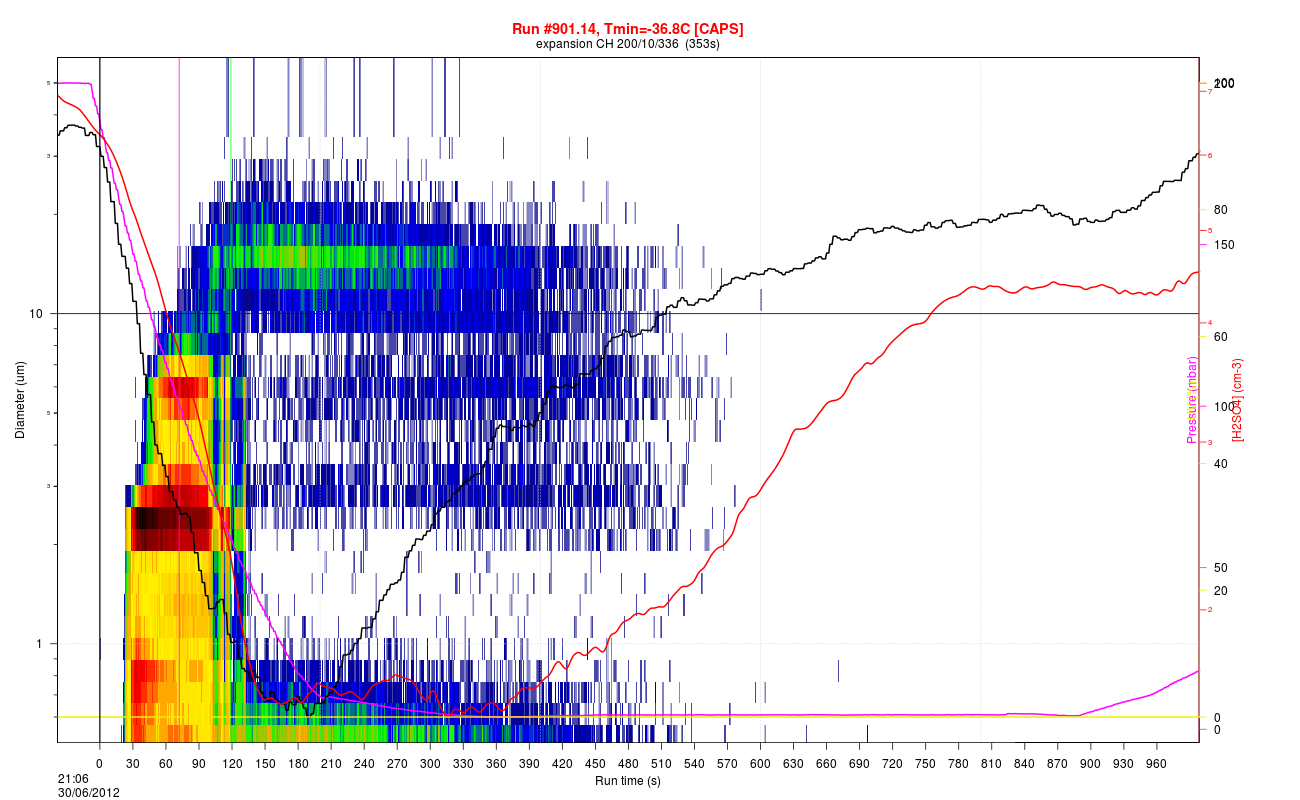
\includegraphics[scale=0.5]{runs_for_talk01.png} 
\caption{show an example picture}
\end{figure}
\end{frame}




